\begin{figure}[h]
    \centering
    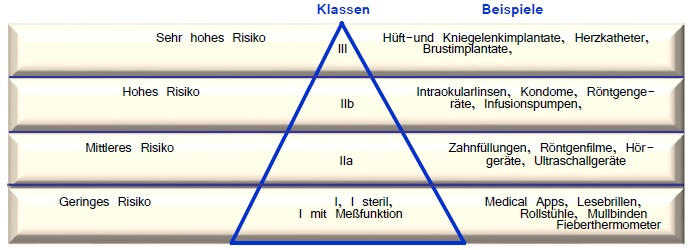
\includegraphics[width=1.0\textwidth]{images/Risikoklassen.jpg}
    \caption{\label{fig:Marktzugangsregelung}
        Risikoklassen
        \protect\cite{Marktzugangsregelung}
    }
\end{figure}
Medizinprodukte wie Röntgengeräte, Implantate, Sehhilfen, Herzschrittmacher, 
Infusionen und Software sind Produkte, die einen bestimmten medizinischen Nutzen am Menschen haben\cite{Marktzugangsregelung}.
Es wird nicht zwischen physikalischen Geräten mit eingebetteter Software und Geräten, die selbst die Software sind, unterschieden. 
Software als Medizinprodukt (SaMD) wird ebenfalls mit denselben Vorschriften, Richtlinien und Gesetzen entwickelt, sowie medizinische Geräte selbst\cite{AI_in_EU}.\\
Wie in Abbildung~\ref{fig:Marktzugangsregelung} zu sehen, werden Medizinprodukte mit der Klassifizierungsregel in vier Risikoklassen eingeteilt.
Die Regeln für die Anwendung der Klassen I, IIa, IIb und III, 
richten sich nach den Zweckbestimmungen der Produkte und liegen in der Verantwortung der Hersteller\cite{Marktzugangsregelung}. Hier werden strenge Anforderungen an die Medizinprodukthersteller gestellt. 
Medizin der Klasse I ist allerdings davon ausgeschlossen, hier reicht eine Selbsterklärung des Herstellers.
\newpage
\begin{figure}[h]
    \centering
    
\includegraphics[width=1.0\textwidth]{images/Zertifizierungsablauf.jpg}
    \caption{\label{fig:Zertifizierungsablauf}
        Ablauf des Zertifizierungsverfahrens
        \protect\footfullcite{zertifizierungsverfahren}
    }
\end{figure}
In Abbildung~\ref{fig:Zertifizierungsablauf} wird der Verlauf der Zertifizierung von Medizinprodukten in Deutschland von MEDCERT dargestellt.
MEDCERT ist eine Benannte Stelle und Zertifizierungsgesellschaft,
die von der Zentralstelle der Länder für Gesundheitsschutz (ZLG) zertifiziert wurde\cite{Marktzugangsregelung}.
Als ersten Schritt muss der Hersteller bei obengenannter Bennanten Stelle einen Antrag stellen. Wichtige Dokumente wie die QM-Dokumentation,
das Organigramm der Firma,
die Berichte zu internen Audits und gegebenenfalls Produktdokumentationen werden an MEDCERT übergeben.
Diese werden in Schritt zwei von der Bennanten Stelle nach den Normen und Anforderungen geprüft.
Hier wird auf die Medizinprodukteverordnung 2017/745 (MDR), die am 25. Mai 2017 in Kraft trat, zurückgegriffen\cite{Produkteverordnung}.
Diese stellt mit drei Richtlinien  die Ansprüche an die Konformitätsbewertungen von Medizinprodukten.
In Schritt drei und vier wird ein Termin vereinbart, in dem genau beschrieben wird, welche Bereiche wann geprüft werden.
Anschließend werden in Schritt fünf und sechs die eingereichten Korrekturmaßnahmen beurteilt und der Zertifikatstext abgestimmt.
In Schritt sieben wird das gesamte Zertifizierungsverfahren bewertet.
Das erfolgreiche Durchlaufen des Verfahrens der Benannten Stelle stellt sicher,
dass das Medizinprodukt alle geltenden Anforderungen erfüllt
und die Hersteller für ihr Medizinprodukt nun die entsprechende CE-Kennzeichnung bekommen\cite{AI_in_EU}.
Schritt neun in Abbildung~\ref{fig:Zertifizierungsablauf} zeigt, dass nun ein jährliches Überwachungsaudit folgt.
Die Medizinprodukte entwickeln sich ständig weiter, werden verbessert und erneuert. 
Diese Änderungen müssen laufend von der Benannten Stelle überprüft und genehmigt werden,
sofern vorgeschriebene Anforderungen beeinträchtigt werden.
Laufende Richtlinien werden immer wieder mit neuen Verordnungen korrigiert und ergänzt. 
Normungsgremien wie die International Organization for Standardization (ISO) und die International Electrotechnical Commission (IEC) sowie europäische Normungsorganisationen bekräftigen europäische Normen, die im Folgenden erklärt werden. 
Die europäische Normen beinhalten die benötigten rechtlichen Anforderungen für die jeweiligen medizinischen Produkte. Den Herstellern steht es frei, sich an den Normen zu orientieren. Jedoch kann durch Einhaltung der Normen die Konformität nachgewiesen werden\cite{AI_in_EU}.\\
Einige ISO und IEC Normen treffen auf die regulierenden Anforderungen zu.
So werden die Qualitätsanforderungen für die Entwicklung von Medizinprodukten weitestgehend durch die harmonisierte Norm ISO 13485 bestimmt\cite{iso13485}. 
Um für die Sicherheit der Menschen bei klinischer Prüfung von Medizinprodukten zu sorgen, dient die Norm ISO 14155\cite{iso14155}.
Die Norm ISO 14971 ist für den Risikomanagementprozess von Medizinprodukten verantwortlich\cite{iso14971}.
Außerdem folgende drei IEC Normen.
Der Software Lebenszyklus von Medizinprodukten fällt unter die Norm IEC 62304\cite{iec62304}. 
Anwendung der Gebrauchstauglichkeit, durch Entwicklungsprozesse,
auf Medizinprodukte lässt sich auf die Norm IEC 62366-1 zurückführen\cite{iec623661}. 
Die Norm IEC 82304-1 beschäftigt sich mit allgemeinen Anforderungen für die Produktsicherheit\cite{iec823041}.